\chapter{Herausforderungen und Ausblick} % Main chapter title
\label{Probleme} % For referencing the chapter elsewhere, use \ref{Chapter1} 

\section{Einleitung}

Bei der Umsetzung dieses Projekts haben sich insbesondere aus Perspektive eines Softwareentwicklers einige neue Herausforderungen gestellt, die sich bei der imperativen Programmierung üblicherweise nicht ergeben (z. B. die grundsätzliche parallele Signalverarbeitung).

Auf einige bestimmte Probleme, mit denen das Team konfrontiert wurde, soll an dieser Stelle gesondert eingegangen werden.

Außerdem sind mehrere Wege denkbar, das entwickelte CPU-Design künftig weiterzuentwickeln. Darunter sind solche, die die Funktionalität erweitern und solche, die das bestehende Design optimieren. Auch auf diese möglichen Entwicklungen soll hier ein kurzer Ausblick gegeben werden.

%----------------------------------------------------------------------------------------
\section{RAM}

In Kapitel~\ref{Umsetzung} wurden Aufbau und Funktionsweise des Hauptspeichers und des RAM-Controllers bereits näher erläutert.
An dieser Stelle sollen nun einige Schwierigkeiten, die während der Implementierung auftraten, und die daraus resultierenden Überlegungen beschrieben werden.

\paragraph{Speicherausrichtung.} 
Ein Speicherzugriff auf $N$ Byte gilt als ausgerichtet, wenn die Startadresse dieser $N$ Byte ein ganzzahliges Vielfaches von $N$ ist~\cite[S. 96/97]{Hennessy}.
Findet z. B. ein Speicherzugriff mit der Breite von 32-Bit auf eine Adresse statt, die nicht ausgerichtet ist, die also kein ganzzahliges Vielfaches von 4 ist, ergibt sich folgendes Problem:
Nicht alle vier Byte des gesuchten Wortes befinden sich unter der gleichen (Wort-)Adresse im Speicher und können daher nicht innerhalb eines einzelnen Zugriffs erreicht werden.

Möchte man diese Art Operation unterstützen, wäre es z. B. denkbar, jeden Zugriff, der mehr als ein Byte umfasst, in eine entsprechende Anzahl von Byte-Zugriffen umzuwandeln, was sich allerdings negativ auf die Performance der CPU auswirken würde.
Außerdem garantiert die RISC-V-Spezifikation nur für ausgerichtete Zugriffe Atomarität, wohingegen bei unausgerichteten Zugriffen zusätzliche Vorkehrungen zu treffen sind~\cite[S. 18]{RISC}.

Der vorliegende RAM-Controller unterstützt unausgerichtete Zugriffe nicht, mit dem Vorteil, dass alle Maschinenbefehle nur zwei Takte zur Ausführung benötigen.
Ein entsprechender Speicherzugriff wird hier also unterbunden, d.h. der Maschinenbefehl wird ignoriert und hat keinerlei Auswirkung.

Umgesetzt wurde dies wie folgt:\\
Bei einem nicht ausgerichteten Schreibzugriff wird der Schreibvorgang nicht unterbrochen, allerdings wird in die jeweilige Speicherstelle der ursprünglich dort enthaltene Wert zurückgeschrieben.
Somit wird der Speicher nicht verändert.\\
Wird dagegen lesend auf eine nicht ausgerichtete Adresse zugegriffen, sendet der RAM-Controller über seinen \textit{dsbl\_wr\_reg}-Port ein Signal an den Dekodierer, der diese Information (\textit{en\_write = false}) an die Registerbank weiterleitet und somit einen Schreibzugriff auf das Register unterbindet, in das der zu lesende Wert aus dem RAM ursprünglich geschrieben werden sollte.

\paragraph{Schreibprozess.} 
Da auf den Hauptspeicher nur ein 32-Bit breiter Zugriff möglich ist, muss der RAM-Controller vor einem Schreibzugriff der Breite 8- oder 16-Bit die adressierte Speicherstelle lesen, um diese verändern und anschließend zurückschreiben zu können~(siehe Kapitel \ref{subsec:RAM}).
Herausforderung bei der Umsetzung dieser Maschineninstruktionen war es, diese in zwei Takten durchführen zu können, um die Anzahl der Takte pro Instruktion nicht erhöhen zu müssen.
Abbildung~\ref{fig:write} zeigt beispielhaft, wie ein Schreibprozess in den RAM durchgeführt wird.
Links sieht man die Namen der entsprechenden Ports und Signale, während rechts deren Werte zum jeweiligen Zeitpunkt (siehe Taktsignal \textit{s\_clk}) dargestellt sind.

\begin{figure}[htpb]
    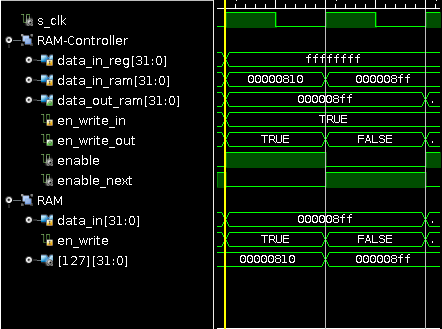
\includegraphics[width=\textwidth]{Figures/write.png}
    \caption{Umsetzung eines Schreibzugriffs in den Speicher}
    \label{fig:write}
\end{figure}

In diesem Beispiel soll ein Byte in den Speicher geschrieben werden:\\
Der RAM-Controller erhält ein Wort von der Registerbank (\textit{data\_in\_reg}), dessen niederwertigstes Byte in den Speicher geschrieben werden soll (in diesem Fall wiederum an die Position des niederwertigsten Bytes).
Gleichzeitig liest er den Wert aus der Speicherstelle, die adressiert wird  (\textit{data\_in\_ram}), um diese mit dem Registerwert zu modifizieren und in den Speicher zurückzuschreiben (\textit{data\_out\_ram}).
Vom Dekoder erhält der RAM-Controller die Information, dass ein Schreibzugriff auf den RAM erforderlich ist (\textit{en\_write\_in}), welche er direkt an den RAM weiterleitet (\textit{en\_write\_out}).
Dieser erhält den Schreibbefehl (\textit{en\_write}) allerdings kurz nach einer steigenden Taktflanke (siehe \textit{s\_clk}), weswegen der eigentliche Schreibvorgang erst im zweiten Takt erfolgt.
Um einen weiteren Schreibzugriff im nächsten Takt zu verhindern, setzt der RAM-Controller das \textit{en\_write\_out}-Signal  mit Hilfe zweier umschaltender Signale (\textit{enable} und \textit{enable\_next}) auf \textit{FALSE}.



\section{Pipelining}
In der vorliegenden Implementierung wurde aus Zeitgründen auf die Umsetzung des sog. Pipelining verzichtet. 
Trotzdem soll hier kurz auf die Grundlagen dieser Technik und deren Voraussetzungen eingegangen werden.
Für eine detaillierte Auseinandersetzung mit diesem Thema wird an dieser Stelle auf weiterführende Literatur verwiesen~\cite[A-2 ff.]{Hennessy}

Pipelining ist ein Verfahren, mit dessen Hilfe die Performance einer CPU verbessert werden kann.
Statt Maschineninstruktionen nacheinander auszuführen, werden diese in Teilaufgaben zerlegt, wodurch es möglich ist, während eines Taktzyklus Befehle parallel abzuarbeiten.
Die Ausführungszeit eines einzelnen Befehls kann dadurch zwar durchaus länger werden, allerdings ist es möglich, insgesamt mehr Instruktionen pro Takt abzuarbeiten.
Klassische Pipeline-Stufen sind z. B.:
\begin{itemize}
    \item Instruction fetch - Laden des Maschinenbefehls
    \item Instruction decode - Dekodieren des Maschinenbefehls
    \item Execute - Ausführen einer Rechenoperation
    \item Memory Access - Zugriff auf den Speicher (bei LOAD- und STORE-Befehlen)
    \item Write back - Zurückschreiben des Ergebnisses in den Speicher
\end{itemize}

Um Pipelining in das vorliegende CPU-Design zu integrieren, wäre es also notwendig die Bearbeitung eines Maschinenbefehls in eindeutig abgegrenzte Stufen zu unterteilen. 
Außerdem müssten die Ergebnisse jeder Stufe in dafür vorgesehene Register zwischengespeichert werden, um diese der jeweils nächsten Phase zur Verfügung zu stellen.

\section{Übersetzen von C-Programmen}
Für die vorliegende CPU ist es zwar möglich Assemblerprogramme zu übersetzen und in den RAM zu laden~(siehe Kapitel \ref{ram-init}), allerdings muss dabei manuell für die korrekte Anordnung der Daten gesorgt werden.
Aus diesem Grund wurde über die Möglichkeit diskutiert, C-Programme zu übersetzen und ohne zusätzliche Vorkehrungen in den Speicher zu laden und auszuführen.
Tatsächlich existiert mit dem RISC-V-GCC\footnote{https://github.com/riscv/riscv-gnu-toolchain (08.03.2017)} bereits ein Compiler für die vorliegende Architektur, allerdings fehlt für das erwähnte Vorhaben eine Ausführungsumgebung (z. B. ein Betriebssystem), die die kompilierte Datei korrekt in den Speicher lädt.

Zwar wurde der naive Versuch unternommen, ein ausführbares C-Programm im ELF-Format (\textit{Executable and Linkable Format}) fast unverändert in den Speicher abzubilden und über kleine Anpassungen den \textit{entry point}, also die Adresse an der die eigentliche Programmausführung beginnt, anzuspringen.
Allerdings folgte die Erkenntnis, dass sich dieses Thema als wesentlich komplexer darstellt als ursprünglich angenommen und damit eine Umsetzung weiterer Recherchen bedarf,~\cite[S. 9 ff.]{elf} auf die im Rahmen dieses Projekts aus Zeitgründen verzichtet wurde.


\section{Erweiterungen des Befehlssatzes}

Aufgrund der flexiblen Erweiterbarkeit der RISC-V-Architektur (siehe
Kapitel \ref{sec:erweiterung}) und des modularen Aufbaus dieses Projekts
sind zusätzliche Instruktionen, die über den RISC-V-Basisbefehlssatz
hinausgehen, verhältnismäßig einfach hinzuzufügen. In der
RISC-V-Spezifikation sind beispielsweise Befehlssatzerweiterungen für
Gleitkommaarithmetik, mehrere Privilegierungsebenen, atomare Befehle für
Multikernprozessoren, aber auch für Bitmanipulation und
Vektoroperationen vorgesehen. \cite[S. 4f.]{RISC} Diese Erweiterungen
können je nach individueller Anforderungen dem Basisbefehlssatz hinzugefügt werden.
 
Denkbar wäre es außerdem, das CPU-Design über RISC-V-Standards hinaus individuell zu erweitern, indem eigene Maschinenbefehle definiert werden, die auf spezielle Anwendungsgebiete zugeschnitten sind.



